\documentclass[tikz,border=15pt]{standalone}
\usepackage{amsmath,amssymb}
\usetikzlibrary{decorations.pathreplacing, calc, shadows, arrows.meta}
\usetikzlibrary{decorations.pathreplacing, calc, shadows, arrows.meta, positioning}

\usepackage[T1]{fontenc}
\usepackage[utf8]{inputenc}
\usepackage{newpxtext,newpxmath}
\usepackage{sectsty}

% Define the color palette
\definecolor{accent}{RGB}{20, 80, 180}       % Blue for Information/Message Space
\definecolor{softaccent}{RGB}{230, 240, 255} 
\definecolor{parity}{RGB}{210, 80, 30}       % Orange for Parity Space
\definecolor{softparity}{RGB}{255, 235, 225} 
\definecolor{ambient}{RGB}{244, 246, 248}    % Gray for Ambient Space
\definecolor{subspace}{RGB}{240, 230, 250}   % Purple tint for the Code Subspace
\definecolor{subspacedraw}{RGB}{140, 80, 180}

\newcommand{\F}{\mathbb{F}}
\newcommand{\code}{\mathcal{C}}
\newcommand{\vect}[1]{\mathbf{#1}}
\newcommand{\id}{\operatorname{id}}

\begin{document}
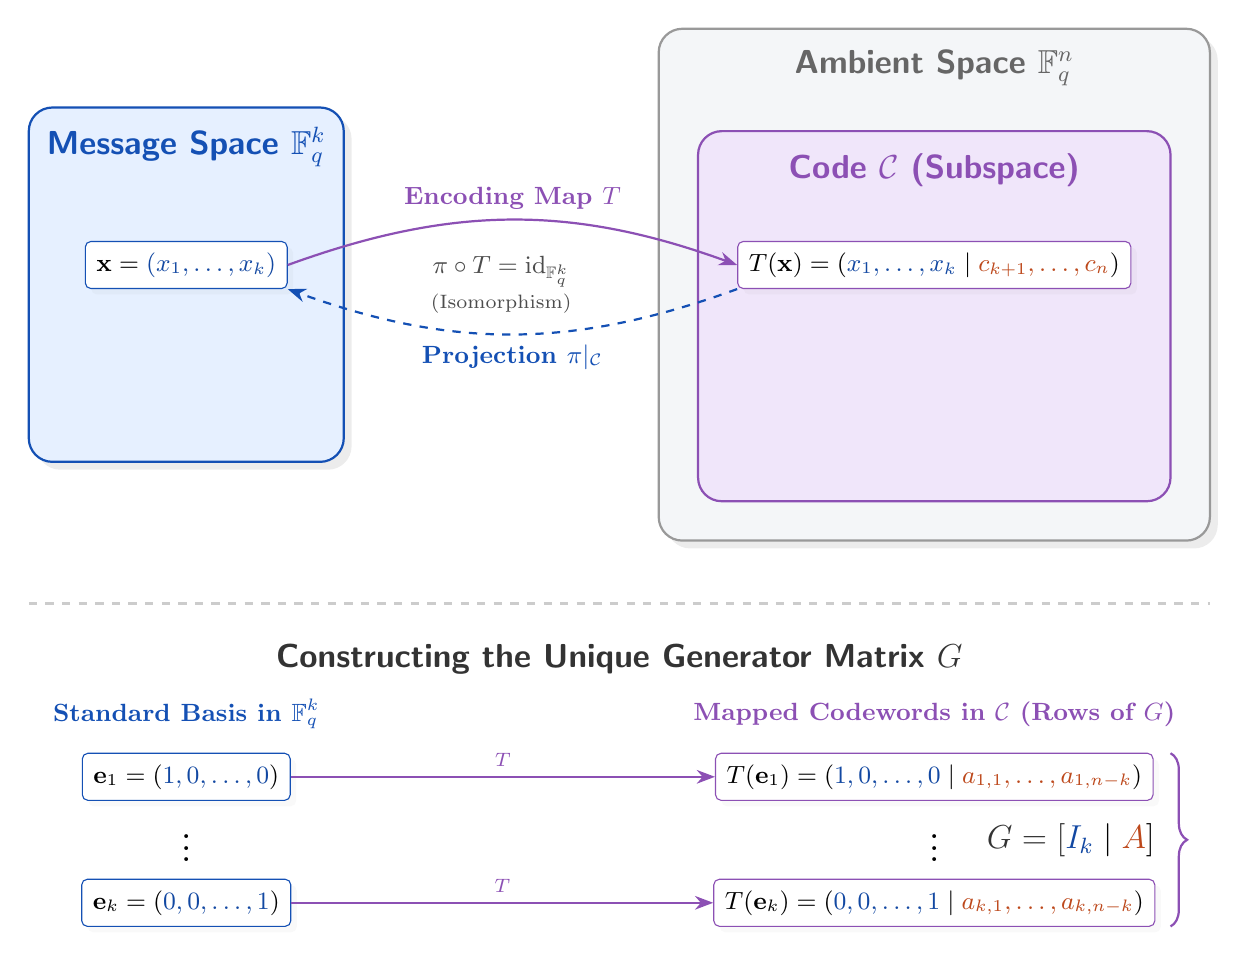
\begin{tikzpicture}[
	>=Stealth,
	font=\sffamily,
	% Styles
	spacebox/.style={thick, rounded corners=3mm, drop shadow={opacity=0.15, shadow xshift=1mm, shadow yshift=-1mm}},
	labeltext/.style={text=black!85, font=\small},
	header/.style={font=\bfseries\sffamily\large},
	coordbox/.style={fill=white, draw=black!30, rounded corners=2pt, inner sep=4pt, font=\small, drop shadow={opacity=0.05}},
	infotext/.style={text=accent!90!black},
	paritytext/.style={text=parity!90!black}
	]
	
	% ==========================================
	% TOP HALF: The Isomorphism T and \pi
	% ==========================================
	
	% Left Space: F_q^k (Message Space)
	\draw[draw=accent, fill=softaccent, spacebox] (0, 0) rectangle (4, 4.5);
	\node[header, text=accent] at (2, 4.0) {Message Space $\F_q^k$};
	
	% Right Space: F_q^n (Ambient Space)
	\draw[draw=black!40, fill=ambient, spacebox] (8, -1) rectangle (15, 5.5);
	\node[header, text=black!60] at (11.5, 5.0) {Ambient Space $\F_q^n$};
	
	% Code Subspace inside F_q^n
	\draw[draw=subspacedraw, fill=subspace, thick, rounded corners=3mm] (8.5, -0.5) rectangle (14.5, 4.2);
	\node[header, text=subspacedraw] at (11.5, 3.7) {Code $\code$ (Subspace)};
	
	% Vector x in F_q^k
	\node[coordbox, draw=accent] (vecX) at (2, 2.5) {$\vect{x} = \color{accent!90!black}(x_1, \dots, x_k)$};
	
	% Vector T(x) in C
	\node[coordbox, draw=subspacedraw] (vecTx) at (11.5, 2.5) {$T(\vect{x}) = (\color{accent!90!black}x_1, \dots, x_k\color{black} \mid \color{parity!90!black}c_{k+1}, \dots, c_n\color{black})$};
	
	% Arrows for T and \pi
	% 1. Encoding Map T
	\draw[->, subspacedraw, thick] (vecX.east) to[bend left=20] 
	node[midway, above, font=\small\bfseries] {Encoding Map $T$} (vecTx.west);
	
	% 2. Projection \pi
	\draw[->, accent, thick, dashed] (vecTx.south west) to[bend left=20] 
	node[midway, below, font=\small\bfseries] {Projection $\pi|_\code$} (vecX.south east);
	
	% Cycle node showing Identity
	\node[labeltext, text=black!70, align=center] at (6, 2.25) {$\pi \circ T = \id_{\F_q^k}$\\[0.5ex] \scriptsize (Isomorphism)};
	
	% ==========================================
	% BOTTOM HALF: Standard Basis to Generator Matrix
	% ==========================================
	
	% Separator Line
	\draw[black!20, thick, dashed] (0, -1.8) -- (15, -1.8);
	
	% Title for Bottom Section
	\node[header, text=black!80] at (7.5, -2.5) {Constructing the Unique Generator Matrix $G$};
	
	% Standard Basis in F_q^k
	\node[labeltext, font=\bfseries\small, text=accent] at (2, -3.2) {Standard Basis in $\F_q^k$};
	
	\node[coordbox, draw=accent] (e1) at (2, -4.0) {$\vect{e}_1 = (\color{accent!90!black}1, 0, \dots, 0\color{black})$};
	\node[font=\Large] (vdots1) at (2, -4.8) {$\vdots$};
	\node[coordbox, draw=accent] (ek) at (2, -5.6) {$\vect{e}_k = (\color{accent!90!black}0, 0, \dots, 1\color{black})$};
	
	% Mapped Basis in C (Rows of G)
	\node[labeltext, font=\bfseries\small, text=subspacedraw] at (11.5, -3.2) {Mapped Codewords in $\code$ (Rows of $G$)};
	
	\node[coordbox, draw=subspacedraw] (Te1) at (11.5, -4.0) {$T(\vect{e}_1) = (\color{accent!90!black}1, 0, \dots, 0\color{black} \mid \color{parity!90!black}a_{1,1}, \dots, a_{1,n-k}\color{black})$};
	\node[font=\Large] (vdots2) at (11.5, -4.8) {$\vdots$};
	\node[coordbox, draw=subspacedraw] (Tek) at (11.5, -5.6) {$T(\vect{e}_k) = (\color{accent!90!black}0, 0, \dots, 1\color{black} \mid \color{parity!90!black}a_{k,1}, \dots, a_{k,n-k}\color{black})$};
	
	% Arrows T
	\draw[->, subspacedraw, thick] (e1.east) -- node[above, font=\scriptsize] {$T$} (Te1.west);
	\draw[->, subspacedraw, thick] (ek.east) -- node[above, font=\scriptsize] {$T$} (Tek.west);
	
	% Final G Matrix Representation
	\draw[decorate, decoration={brace, amplitude=6pt}, thick, subspacedraw] (14.5, -3.7) -- (14.5, -5.9);
	\node[right=10pt of vdots2, font=\large\bfseries, text=black!80] {$G = [\color{accent!90!black}I_k\color{black} \mid \color{parity!90!black}A\color{black}]$};
	
\end{tikzpicture}
\end{document}